% This LaTeX document needs to be compiled with XeLaTeX.
\documentclass[10pt]{article}
\usepackage[utf8]{inputenc}
\usepackage{graphicx}
\usepackage[export]{adjustbox}
\graphicspath{ {./images/} }
\usepackage{amsmath}
\usepackage{amsfonts}
\usepackage{amssymb}
\usepackage[version=4]{mhchem}
\usepackage{stmaryrd}
\usepackage{bbold}
\usepackage[fallback]{xeCJK}
\usepackage{polyglossia}
\usepackage{fontspec}
\setCJKmainfont{Noto Serif CJK KR}

\setmainlanguage{polish}
\setmainfont{CMU Serif}

\title{Egzamin maturalny }

\author{}
\date{}


\begin{document}
\maketitle
\begin{center}
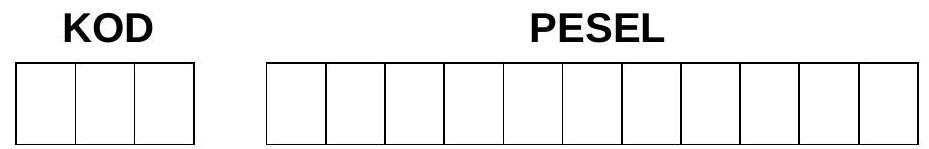
\includegraphics[max width=\textwidth]{2024_11_21_daeb5e5efb43dd4cb535g-01}
\end{center}

\section*{Miejsce na naklejkę.}
Sprawdź, czy kod na naklejce to M-100.

Jeżeli tak - przyklej naklejkę. Jeżeli nie - zgłoś to nauczycielowi.

\section*{Formuła 2023}
\section*{MATEMATYKA}
\section*{Poziom podstawowy}
Symbol arkusza\\
MMAP-P0-100-2405

\section*{DATA: 8 maja 2024 r. \\
 GoDZINA ROZPOCzĘCIA: 9:00 \\
 CZAS trWANIA: \(\mathbf{1 8 0}\) minut}
\begin{center}
\begin{tabular}{|l|}
\hline
WYPEŁNIA ZESPÓŁ NADZORUJĄCY \\
\hline
Uprawnienia zdającego do: \\
\(\square\) dostosowania zasad oceniania \\
\(\square\) dostosowania w zw. z dyskalkulią \\
\(\square\) nieprzenoszenia odpowiedzi na kartę. \\
\hline
\end{tabular}
\end{center}

LICZBA PUNKTÓW DO UZYSKANIA: 46

Przed rozpoczęciem pracy z arkuszem egzaminacyjnym

\begin{enumerate}
  \item Sprawdź, czy nauczyciel przekazał Ci właściwy arkusz egzaminacyjny, tj. arkusz we właściwej formule, z właściwego przedmiotu na właściwym poziomie.
  \item Jeżeli przekazano Ci niewłaściwy arkusz - natychmiast zgłoś to nauczycielowi Nie rozrywaj banderol.
  \item Jeżeli przekazano Ci właściwy arkusz - rozerwij banderole po otrzymaniu takiego polecenia od nauczyciela. Zapoznaj się z instrukcją na stronie 2.\\

\includegraphics[max width=\textwidth, center]{2024_11_21_daeb5e5efb43dd4cb535g-02}
\end{enumerate}

\section*{Instrukcja dla zdającego}
\begin{enumerate}
  \item Sprawdź, czy arkusz egzaminacyjny zawiera 30 stron (zadania 1-31). Ewentualny brak zgłoś przewodniczącemu zespołu nadzorującego egzamin.
  \item Na pierwszej stronie arkusza oraz na karcie odpowiedzi wpisz swój numer PESEL i przyklej naklejkę z kodem.
  \item Symbol 回回/zamieszczony w nagłówku zadania oznacza, że rozwiązanie zadania zamkniętego musisz przenieść na kartę odpowiedzi. Ocenie podlegają wyłącznie odpowiedzi zaznaczone na karcie odpowiedzi.
  \item Odpowiedzi do zadań zamkniętych zaznacz na karcie odpowiedzi w części karty przeznaczonej dla zdającego. Zamaluj \(\square\) pola do tego przeznaczone. Błędne zaznaczenie otocz kółkiem ( ) zaznacz właściwe.
  \item Pamiętaj, że pominięcie argumentacji lub istotnych obliczeń w rozwiązaniu zadania otwartego może spowodować, że za to rozwiązanie nie otrzymasz pełnej liczby punktów.
  \item Rozwiązania zadań i odpowiedzi wpisuj w miejscu na to przeznaczonym.
  \item Pisz czytelnie i używaj tylko długopisu lub pióra z czarnym tuszem lub atramentem.
  \item Nie używaj korektora, a błędne zapisy wyraźnie przekreśl.
  \item Nie wpisuj żadnych znaków w tabelkach przeznaczonych dla egzaminatora. Tabelki umieszczone są na marginesie przy odpowiednich zadaniach.
  \item Pamiętaj, że zapisy w brudnopisie nie będą oceniane.
  \item Możesz korzystać z Wybranych wzorów matematycznych, cyrkla i linijki oraz kalkulatora prostego. Upewnij się, czy przekazano Ci broszurę z okładką taką jak widoczna poniżej.\\
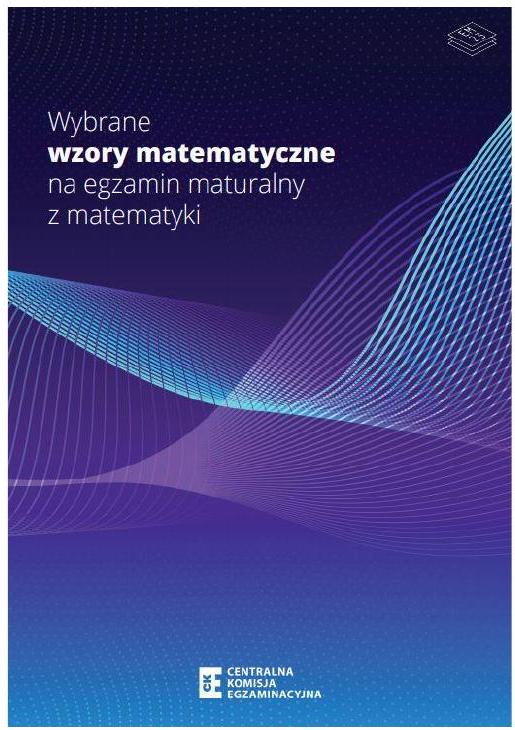
\includegraphics[max width=\textwidth, center]{2024_11_21_daeb5e5efb43dd4cb535g-02(1)}
\end{enumerate}

\section*{Zadania egzaminacyjne są wydrukowane na następnych stronach.}
Zadanie 1. (0-1) 回回\\
Dana jest nierówność

\[
|x-1| \geq 3
\]

Na którym rysunku poprawnie zaznaczono na osi liczbowej zbiór wszystkich liczb rzeczywistych spełniających powyższą nierówność? Wybierz właściwą odpowiedź spośród podanych.\\
A.\\
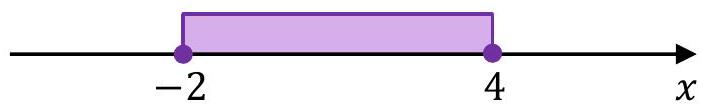
\includegraphics[max width=\textwidth, center]{2024_11_21_daeb5e5efb43dd4cb535g-04(2)}\\
B.\\
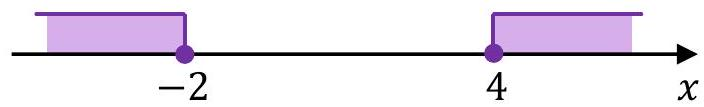
\includegraphics[max width=\textwidth, center]{2024_11_21_daeb5e5efb43dd4cb535g-04}\\
C.\\
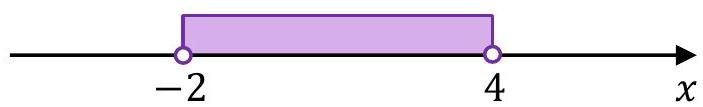
\includegraphics[max width=\textwidth, center]{2024_11_21_daeb5e5efb43dd4cb535g-04(1)}\\
D.\\
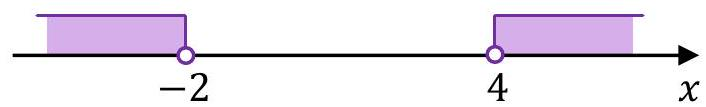
\includegraphics[max width=\textwidth, center]{2024_11_21_daeb5e5efb43dd4cb535g-04(3)}

\begin{center}
\begin{tabular}{|c|c|c|c|c|c|c|c|c|c|c|c|c|c|c|c|c|c|c|c|c|c|c|}
\hline
\multicolumn{4}{|l|}{Brudnopis} &  &  &  &  &  &  &  &  &  &  &  &  &  &  &  &  &  &  &  \\
\hline
 &  &  &  &  &  &  &  &  &  &  &  &  &  &  &  &  &  &  &  &  &  &  \\
\hline
 &  &  &  &  &  &  &  &  &  &  &  &  &  &  &  &  &  &  &  &  &  &  \\
\hline
 &  &  &  &  &  &  &  &  &  &  &  &  &  &  &  &  &  &  &  &  &  &  \\
\hline
 &  &  &  &  &  &  &  &  &  &  &  &  &  &  &  &  &  &  &  &  &  &  \\
\hline
 &  &  &  &  &  &  &  &  &  &  &  &  &  &  &  &  &  &  &  &  &  &  \\
\hline
 &  &  &  &  &  &  &  &  &  &  &  &  &  &  &  &  &  &  &  &  &  &  \\
\hline
 &  &  &  &  &  &  &  &  &  &  &  &  &  &  &  &  &  &  &  &  &  &  \\
\hline
 &  &  &  &  &  &  &  &  &  &  &  &  &  &  &  &  &  &  &  &  &  &  \\
\hline
\end{tabular}
\end{center}

Zadanie 2. (0-1)\\
Dokończ zdanie. Wybierz właściwą odpowiedź spośród podanych.\\
Liczba \(\left(\frac{1}{16}\right)^{8} \cdot 8^{16}\) jest równa\\
A. \(2^{24}\)\\
B. \(2^{16}\)\\
C. \(2^{12}\)\\
D. \(2^{8}\)\\

\includegraphics[max width=\textwidth, center]{2024_11_21_daeb5e5efb43dd4cb535g-04(4)}

Zadanie 3. (0-2)\\
Wykaż, że dla każdej liczby naturalnej \(n \geq 1\) liczba \(n^{2}+(n+1)^{2}+(n+2)^{2}\) przy dzieleniu przez 3 daje resztę 2.\\

\includegraphics[max width=\textwidth, center]{2024_11_21_daeb5e5efb43dd4cb535g-05}

Zadanie 4. (0-1)\\
Dokończ zdanie. Wybierz właściwą odpowiedź spośród podanych.

Liczba \(\log _{\sqrt{3}} 9\) jest równa\\
A. 2\\
B. 3\\
C. 4\\
D. 9

\begin{center}
\begin{tabular}{|c|c|c|c|c|c|c|c|c|c|c|c|c|c|c|c|c|c|c|c|c|c|c|c|c|c|c|c|c|c|c|}
\hline
B & d & nop & pis &  &  &  &  &  &  &  &  &  &  &  &  &  &  &  &  &  &  &  &  &  &  &  &  &  &  &  \\
\hline
 &  &  &  &  &  &  &  &  &  &  &  &  &  &  &  &  &  &  &  &  &  &  &  &  &  &  &  &  &  &  \\
\hline
 &  &  &  &  &  &  &  &  &  &  &  &  &  &  &  &  &  &  &  &  &  &  &  &  &  &  &  &  &  &  \\
\hline
 &  &  &  &  &  &  &  &  &  &  &  &  &  &  &  &  &  &  &  &  &  &  &  &  &  &  &  &  &  &  \\
\hline
 &  &  &  &  &  &  &  &  &  &  &  &  &  &  &  &  &  &  &  &  &  &  &  &  &  &  &  &  &  &  \\
\hline
 &  &  &  &  &  &  &  &  &  &  &  &  &  &  &  &  &  &  &  &  &  &  &  &  &  &  &  &  &  &  \\
\hline
 &  &  &  &  &  &  &  &  &  &  &  &  &  &  &  &  &  &  &  &  &  &  &  &  &  &  &  &  &  &  \\
\hline
 &  &  &  &  &  &  &  &  &  &  &  &  &  &  &  &  &  &  &  &  &  &  &  &  &  &  &  &  &  &  \\
\hline
 &  &  &  &  &  &  &  &  &  &  &  &  &  &  &  &  &  &  &  &  &  &  &  &  &  &  &  &  &  &  \\
\hline
 &  &  &  &  &  &  &  &  &  &  &  &  &  &  &  &  &  &  &  &  &  &  &  &  &  &  &  &  &  &  \\
\hline
 &  &  &  &  &  &  &  &  &  &  &  &  &  &  &  &  &  &  &  &  &  &  &  &  &  &  &  &  &  &  \\
\hline
 &  &  &  &  &  &  &  &  &  &  &  &  &  &  &  &  &  &  &  &  &  &  &  &  &  &  &  &  &  &  \\
\hline
 &  &  &  &  &  &  &  &  &  &  &  &  &  &  &  &  &  &  &  &  &  &  &  &  &  &  &  &  &  &  \\
\hline
 &  &  &  &  &  &  &  &  &  &  &  &  &  &  &  &  &  &  &  &  &  &  &  &  &  &  &  &  &  &  \\
\hline
 &  &  &  &  &  &  &  &  &  &  &  &  &  &  &  &  &  &  &  &  &  &  &  &  &  &  &  &  &  &  \\
\hline
\end{tabular}
\end{center}

\section*{Zadanie 5. (0-1)}
Dokończ zdanie. Wybierz właściwą odpowiedź spośród podanych.

Dla każdej liczby rzeczywistej \(a\) i dla każdej liczby rzeczywistej \(b\) wartość wyrażenia \((2 a+b)^{2}-(2 a-b)^{2}\) jest równa wartości wyrażenia\\
A. \(8 a^{2}\)\\
B. \(8 a b\)\\
C. \(-8 a b\)\\
D. \(2 b^{2}\)\\

\includegraphics[max width=\textwidth, center]{2024_11_21_daeb5e5efb43dd4cb535g-06}

Dokończ zdanie. Wybierz właściwą odpowiedź spośród podanych.\\
Zbiorem wszystkich rozwiązań nierówności

\[
1-\frac{3}{2} x<\frac{2}{3}-x
\]

jest przedział\\
A. \(\left(-\infty,-\frac{2}{3}\right)\)\\
B. \(\left(-\infty, \frac{2}{3}\right)\)\\
C. \(\left(-\frac{2}{3},+\infty\right)\)\\
D. \(\left(\frac{2}{3},+\infty\right)\)

\begin{center}
\begin{tabular}{|c|c|c|c|c|c|c|c|c|c|c|c|c|c|c|c|c|c|c|c|c|c|}
\hline
\multicolumn{4}{|l|}{Brudnopis} &  &  &  &  &  &  &  &  & - &  & - & - &  &  & - &  &  &  \\
\hline
 &  &  &  &  &  &  &  &  &  &  &  &  &  &  &  &  &  &  &  &  &  \\
\hline
 &  &  &  &  &  &  &  &  &  &  &  &  &  &  &  &  &  &  &  &  &  \\
\hline
 &  &  &  &  &  &  &  &  &  &  &  &  &  &  &  &  &  &  &  &  &  \\
\hline
 &  &  &  &  &  &  &  &  &  &  &  &  &  &  &  &  &  &  &  &  &  \\
\hline
 &  &  &  &  &  &  &  &  &  &  &  &  &  &  &  &  &  &  &  &  &  \\
\hline
 &  &  &  &  &  &  &  &  &  &  &  &  &  &  &  &  &  &  &  &  &  \\
\hline
 &  &  &  &  &  &  &  &  &  &  &  &  &  &  &  &  &  &  &  &  &  \\
\hline
 &  &  &  &  &  &  &  &  &  &  &  &  &  &  &  &  &  &  &  &  &  \\
\hline
 &  &  &  &  &  &  &  &  &  &  &  &  &  &  &  &  &  &  &  &  &  \\
\hline
 &  &  &  &  &  &  &  &  &  &  &  &  &  &  &  &  &  &  &  &  &  \\
\hline
\end{tabular}
\end{center}

\section*{Zadanie 7. (0-1)}
Dokończ zdanie. Wybierz właściwą odpowiedź spośród podanych.\\
Równanie \(\frac{x+1}{(x+2)(x-3)}=0 \mathrm{w}\) zbiorze liczb rzeczywistych\\
A. nie ma rozwiązania.\\
B. ma dokładnie jedno rozwiązanie: (-1).\\
C. ma dokładnie dwa rozwiązania: (-2) oraz 3.\\
D. ma dokładnie trzy rozwiązania: \((-1),(-2)\) oraz 3.\\

\includegraphics[max width=\textwidth, center]{2024_11_21_daeb5e5efb43dd4cb535g-07}

Zadanie 8. (0-1) 可\\
Dany jest wielomian \(W(x)=3 x^{3}+6 x^{2}+9 x\).

Oceń prawdziwość poniższych stwierdzeń. Wybierz \(P\), jeśli stwierdzenie jest prawdziwe, albo F - jeśli jest fałszywe.

\begin{center}
\begin{tabular}{|l|l|c|}
\hline
Wielomian \(W\) jest iloczynem wielomianów \(F(x)=3 x\) i \(G(x)=x^{2}+2 x+3\). & \(\mathbf{P}\) & \(\mathbf{F}\) \\
\hline
Liczba \((-1)\) jest rozwiązaniem równania \(W(x)=0\). & \(\mathbf{P}\) & \(\mathbf{F}\) \\
\hline
\end{tabular}
\end{center}

\begin{center}
\begin{tabular}{|c|c|c|c|c|c|c|c|c|c|c|c|c|c|c|c|c|c|c|c|c|c|c|c|c|c|}
\hline
\multicolumn{5}{|l|}{Brudnopis} &  &  &  &  &  &  &  &  &  &  &  &  &  &  &  &  &  &  &  &  &  \\
\hline
 &  &  &  &  &  &  &  &  &  &  &  &  &  &  &  &  &  &  &  &  &  &  &  &  &  \\
\hline
 &  &  &  &  &  &  &  &  &  &  &  &  &  &  &  &  &  &  &  &  &  &  &  &  &  \\
\hline
 &  &  &  &  &  &  &  &  &  &  &  &  &  &  &  &  &  &  &  &  &  &  &  &  &  \\
\hline
 &  &  &  &  &  &  &  &  &  &  &  &  &  &  &  &  &  &  &  &  &  &  &  &  &  \\
\hline
 &  &  &  &  &  &  &  &  &  &  &  &  &  &  &  &  &  &  &  &  &  &  &  &  &  \\
\hline
 &  &  &  &  &  &  &  &  &  &  &  &  &  &  &  &  &  &  &  &  &  &  &  &  &  \\
\hline
 &  &  &  &  &  &  &  &  &  &  &  &  &  &  &  &  &  &  &  &  &  &  &  &  &  \\
\hline
 &  &  &  &  &  &  &  &  &  &  &  &  &  &  &  &  &  &  &  &  &  &  &  &  &  \\
\hline
 &  &  &  &  &  &  &  &  &  &  &  &  &  &  &  &  &  &  &  &  &  &  &  &  &  \\
\hline
 &  &  &  &  &  &  &  &  &  &  &  &  &  &  &  &  &  &  &  &  &  &  &  &  &  \\
\hline
 &  &  &  &  &  &  &  &  &  &  &  &  &  &  &  &  &  &  &  &  &  &  &  &  &  \\
\hline
 &  &  &  &  &  &  &  &  &  &  &  &  &  &  &  &  &  &  &  &  &  &  &  &  &  \\
\hline
 &  &  &  &  &  &  &  &  &  &  &  &  &  &  &  &  &  &  &  &  &  &  &  &  &  \\
\hline
\end{tabular}
\end{center}

Zadanie 9. (0-3)\\
Rozwiąż równanie

\[
x^{3}-2 x^{2}-3 x+6=0
\]

Zapisz obliczenia.\\

\includegraphics[max width=\textwidth, center]{2024_11_21_daeb5e5efb43dd4cb535g-08}\\

\includegraphics[max width=\textwidth, center]{2024_11_21_daeb5e5efb43dd4cb535g-09}

\section*{Zadanie 10. (0-1) 回回}
W październiku 2022 roku założono dwa sady, w których posadzono łącznie 1960 drzew. Po roku stwierdzono, że uschło 5\% drzew w pierwszym sadzie i 10\% drzew w drugim sadzie. Uschnięte drzewa usunięto, a nowych nie dosadzano.\\
Liczba drzew, które pozostały w drugim sadzie, stanowiła 60\% liczby drzew, które pozostały w pierwszym sadzie.\\
Niech \(x\) oraz \(y\) oznaczają liczby drzew posadzonych - odpowiednio - w pierwszym i drugim sadzie.

Dokończ zdanie. Wybierz właściwą odpowiedź spośród podanych.

Układem równań, którego poprawne rozwiązanie prowadzi do obliczenia liczby \(x\) drzew posadzonych w pierwszym sadzie oraz liczby \(y\) drzew posadzonych w drugim sadzie, jest\\
A. \(\left\{\begin{array}{l}x+y=1960 \\ 0,6 \cdot 0,95 x=0,9 y\end{array}\right.\)\\
B. \(\left\{\begin{array}{l}x+y=1960 \\ 0,95 x=0,6 \cdot 0,9 y\end{array}\right.\)\\
C. \(\left\{\begin{array}{l}x+y=1960 \\ 0,05 x=0,6 \cdot 0,1 y\end{array}\right.\)\\
D. \(\left\{\begin{array}{l}x+y=1960 \\ 0,4 \cdot 0,95 x=0,9 y\end{array}\right.\)\\

\includegraphics[max width=\textwidth, center]{2024_11_21_daeb5e5efb43dd4cb535g-10}

\section*{Zadanie 11. (0-1) П丁口.}
Na rysunku, w kartezjańskim układzie współrzędnych \((x, y)\), przedstawiono dwie proste równoległe, które są interpretacją geometryczną jednego z poniższych układów równań A-D.\\
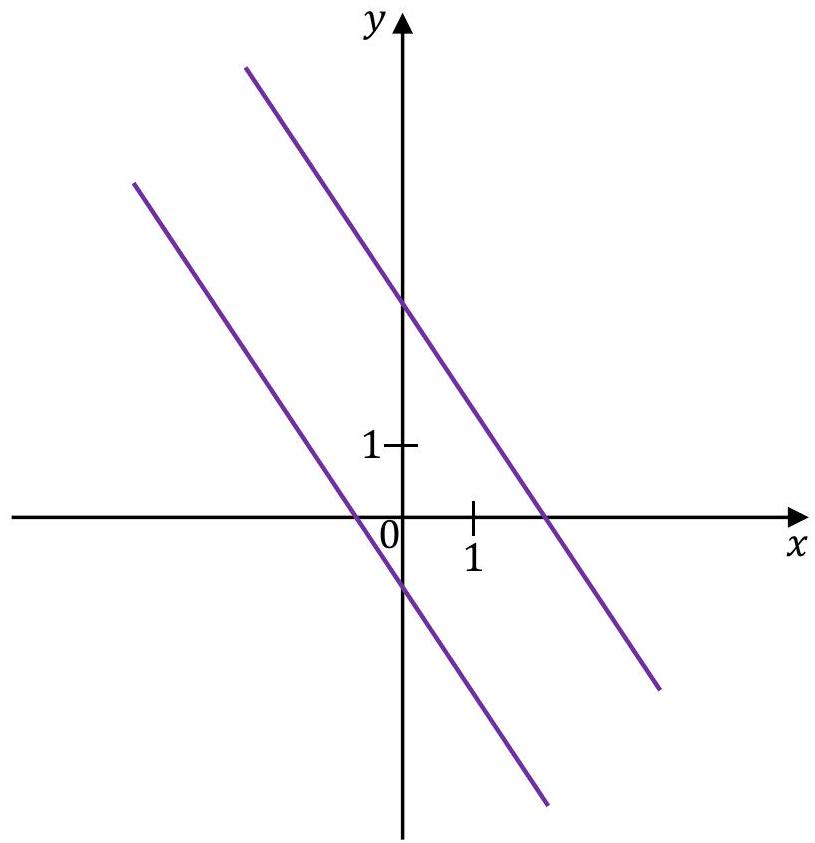
\includegraphics[max width=\textwidth, center]{2024_11_21_daeb5e5efb43dd4cb535g-11(1)}

\section*{Dokończ zdanie. Wybierz właściwą odpowiedź spośród podanych.}
Układem równań, którego interpretację geometryczną przedstawiono na rysunku, jest\\
A. \(\left\{\begin{array}{l}y=-\frac{3}{2} x+3 \\ y=-\frac{3}{2} x-1\end{array}\right.\)\\
B. \(\left\{\begin{array}{l}y=\frac{3}{2} x+3 \\ y=-\frac{2}{3} x-1\end{array}\right.\)\\
C. \(\left\{\begin{array}{l}y=\frac{3}{2} x+3 \\ y=\frac{3}{2} x-1\end{array}\right.\)\\
D. \(\left\{\begin{array}{l}y=-\frac{3}{2} x-3 \\ y=\frac{3}{2} x+1\end{array}\right.\)\\

\includegraphics[max width=\textwidth, center]{2024_11_21_daeb5e5efb43dd4cb535g-11}

Zadanie 12. (0-1) 마미\\
Funkcja liniowa \(f\) jest określona wzorem \(f(x)=(-2 k+3) x+k-1\), gdzie \(k \in \mathbb{R}\).\\
Dokończ zdanie. Wybierz właściwą odpowiedź spośród podanych.\\
Funkcja \(f\) jest malejąca dla każdej liczby \(k\) należącej do przedziału\\
A. \((-\infty, 1)\)\\
B. \(\left(-\infty,-\frac{3}{2}\right)\)\\
C. \((1,+\infty)\)\\
D. \(\left(\frac{3}{2},+\infty\right)\)

\begin{center}
\begin{tabular}{|c|c|c|c|c|c|c|c|c|c|c|c|c|c|c|c|c|c|c|c|c|c|}
\hline
 & Brudn & nopis &  &  &  &  &  &  &  &  &  & - &  & - & - & - &  & - &  &  &  \\
\hline
 &  &  &  &  &  &  &  &  &  &  &  &  &  &  &  &  &  &  &  &  &  \\
\hline
 &  &  &  &  &  &  &  &  &  &  &  &  &  &  &  &  &  &  &  &  &  \\
\hline
 &  &  &  &  &  &  &  &  &  &  &  &  &  &  &  &  &  &  &  &  &  \\
\hline
 &  &  &  &  &  &  &  &  &  &  &  &  &  &  &  &  &  &  &  &  &  \\
\hline
 &  &  &  &  &  &  &  &  &  &  &  &  &  &  &  &  &  &  &  &  &  \\
\hline
 &  &  &  &  &  &  &  &  &  &  &  &  &  &  &  &  &  &  &  &  &  \\
\hline
 &  &  &  &  &  &  &  &  &  &  &  &  &  &  &  &  &  &  &  &  &  \\
\hline
 &  &  &  &  &  &  &  &  &  &  &  &  &  &  &  &  &  &  &  &  &  \\
\hline
 &  &  &  &  &  &  &  &  &  &  &  &  &  &  &  &  &  &  &  &  &  \\
\hline
 &  &  &  &  &  &  &  &  &  &  &  &  &  &  &  &  &  &  &  &  &  \\
\hline
 &  &  &  &  &  &  &  &  &  &  &  &  &  &  &  &  &  &  &  &  &  \\
\hline
\end{tabular}
\end{center}

\section*{Zadanie 13. (0-1) 미미}
Funkcje liniowe \(f\) oraz \(g\), określone wzorami \(f(x)=3 x+6\) oraz \(g(x)=a x+7\), maja to samo miejsce zerowe.

Dokończ zdanie. Wybierz właściwą odpowiedź spośród podanych.\\
Współczynnik \(a\) we wzorze funkcji \(g\) jest równy\\
A. \(\left(-\frac{7}{2}\right)\)\\
B. \(\left(-\frac{2}{7}\right)\)\\
C. \(\frac{2}{7}\)\\
D. \(\frac{7}{2}\)\\

\includegraphics[max width=\textwidth, center]{2024_11_21_daeb5e5efb43dd4cb535g-12}

\section*{Zadanie 14.}
W kartezjańskim układzie współrzędnych \((x, y)\) przedstawiono fragment paraboli, która jest wykresem funkcji kwadratowej \(f\) (zobacz rysunek). Wierzchołek tej paraboli oraz punkty przecięcia paraboli z osiami układu współrzędnych mają obie współzędne całkowite.\\
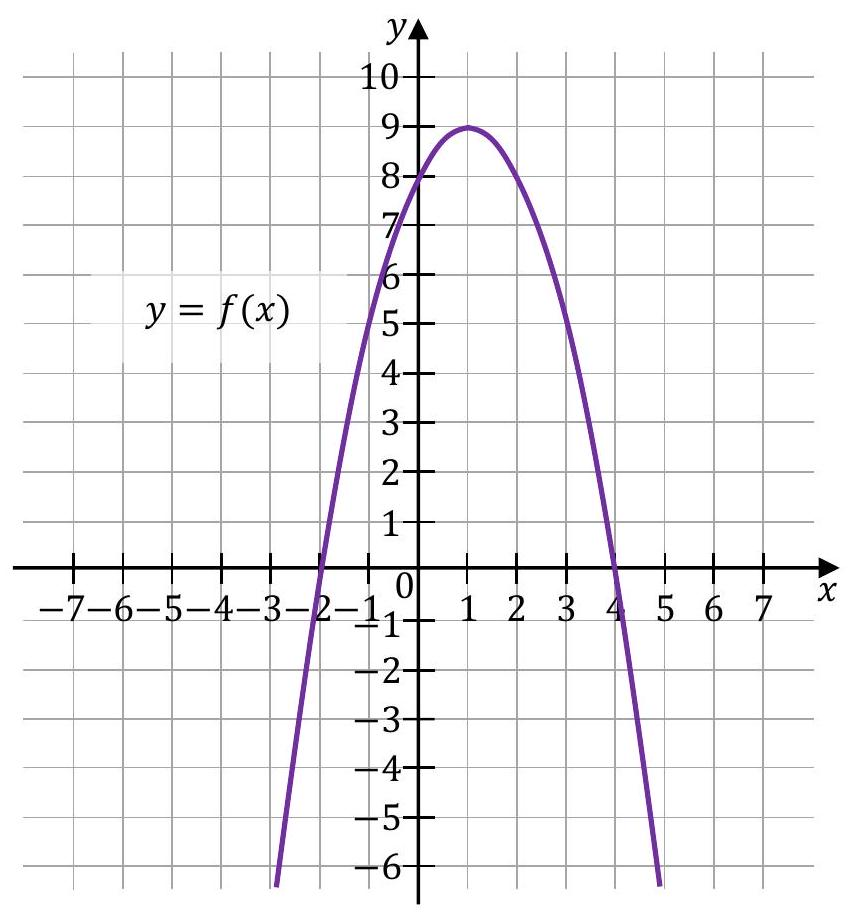
\includegraphics[max width=\textwidth, center]{2024_11_21_daeb5e5efb43dd4cb535g-13(1)}

Zadanie 14.1. (0-1)\\
Uzupełnij poniższe zdanie. Wpisz odpowiedni przedział w wykropkowanym miejscu tak, aby zdanie było prawdziwe.

Zbiorem wszystkich rozwiązań nierówności \(f(x) \geq 0\) jest przedział \(\qquad\) .

\begin{center}
\begin{tabular}{|c|c|c|c|c|c|c|c|c|c|c|c|c|c|c|c|c|c|c|c|c|c|c|c|c|c|}
\hline
\multicolumn{4}{|l|}{Brudnopis} &  &  &  &  &  &  &  &  &  &  &  &  &  &  &  &  &  &  &  &  &  &  \\
\hline
 & - & - &  &  &  &  &  &  &  &  &  &  &  &  &  &  &  &  &  &  &  &  &  &  &  \\
\hline
 &  &  &  &  &  &  &  &  &  &  &  &  &  &  &  &  &  &  &  &  &  &  &  &  &  \\
\hline
 &  &  &  &  &  &  &  &  &  &  &  &  &  &  &  &  &  &  &  &  &  &  &  &  &  \\
\hline
\end{tabular}
\end{center}

\section*{\begin{center}

\includegraphics[max width=\textwidth]{2024_11_21_daeb5e5efb43dd4cb535g-13}
\end{center}}
Dokończ zdanie. Wybierz właściwą odpowiedź spośród podanych.\\
Funkcja kwadratowa \(f\) jest określona wzorem\\
A. \(f(x)=-(x+1)^{2}-9\)\\
B. \(f(x)=-(x-1)^{2}+9\)\\
C. \(f(x)=-(x-1)^{2}-9\)\\
D. \(f(x)=-(x+1)^{2}+9\)

\begin{center}
\begin{tabular}{|l|l|l|l|l|l|l|l|l|l|l|l|l|l|l|l|l|l|l|l|l|l|l|l|l|l|l|l|}
\hline
\multicolumn{2}{|c|}{Brudnopis} &  &  &  &  &  &  &  &  &  &  &  &  &  &  &  &  &  &  &  &  &  &  &  &  &  \\
\hline
\end{tabular}
\end{center}

Zadanie 14.3. (0-1) 미\\
Dokończ zdanie. Wybierz właściwą odpowiedź spośród podanych.\\
Dla funkcji \(f\) prawdziwa jest równość\\
A. \(f(-4)=f(6)\)\\
B. \(f(-4)=f(5)\)\\
C. \(f(-4)=f(4)\)\\
D. \(f(-4)=f(7)\)\\

\includegraphics[max width=\textwidth, center]{2024_11_21_daeb5e5efb43dd4cb535g-14}

\section*{Zadanie 14.4. (0-2)}
Funkcje kwadratowe \(g\) oraz \(h\) są określone za pomocą funkcji \(f\) (zobacz rysunek na stronie 13) następująco: \(g(x)=f(x+3), h(x)=f(-x)\).\\
Na rysunkach A-F przedstawiono, w kartezjańskim układzie współrzędnych \((x, y)\), fragmenty wykresów różnych funkcji - w tym fragment wykresu funkcji \(g\) oraz fragment wykresu funkcji \(h\).

Uzupełnij tabelę. Każdej z funkcji \(\boldsymbol{g}\) oraz \(\boldsymbol{h}\) przyporządkuj fragment jej wykresu. Wpisz w każdą pustą komórkę tabeli właściwą odpowiedź, wybraną spośród oznaczonych literami A-F.

\begin{center}
\begin{tabular}{|l|l|}
\hline
Fragment wykresu funkcji \(y=g(x)\) przedstawiono na rysunku &  \\
\hline
Fragment wykresu funkcji \(y=h(x)\) przedstawiono na rysunku &  \\
\hline
\end{tabular}
\end{center}

A.\\
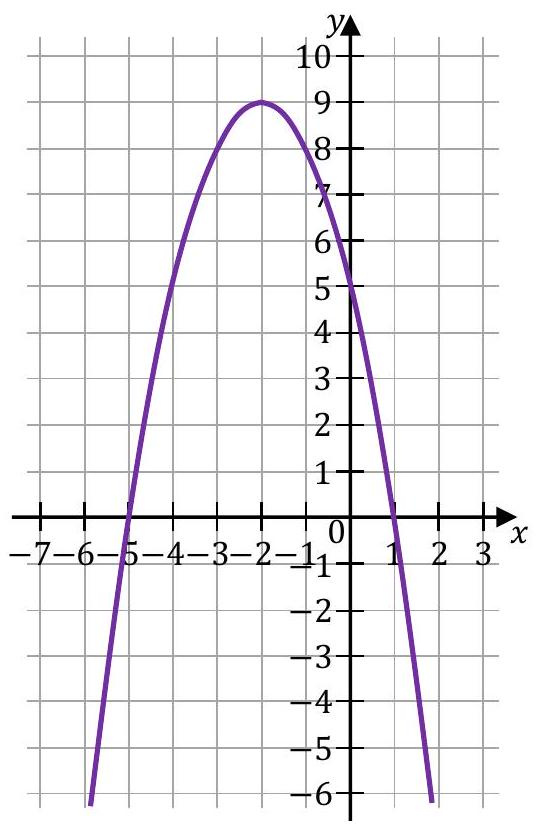
\includegraphics[max width=\textwidth, center]{2024_11_21_daeb5e5efb43dd4cb535g-14(1)}\\
B.\\
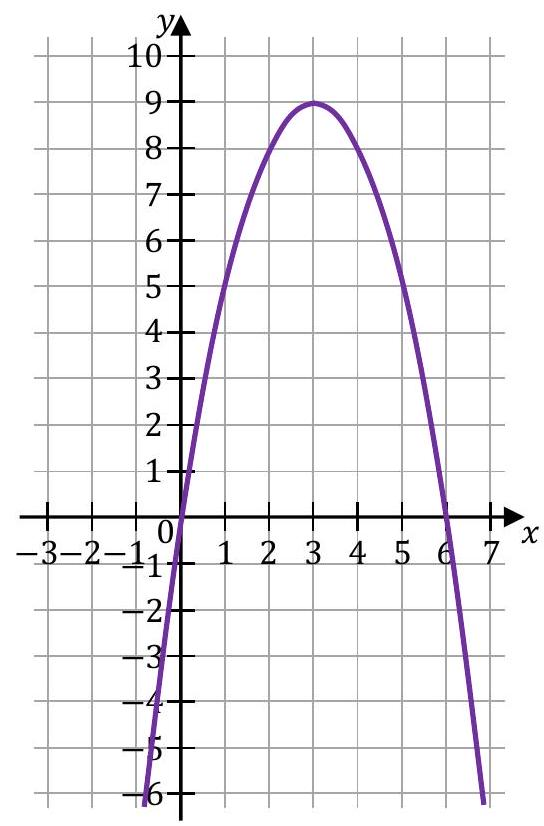
\includegraphics[max width=\textwidth, center]{2024_11_21_daeb5e5efb43dd4cb535g-14(2)}\\
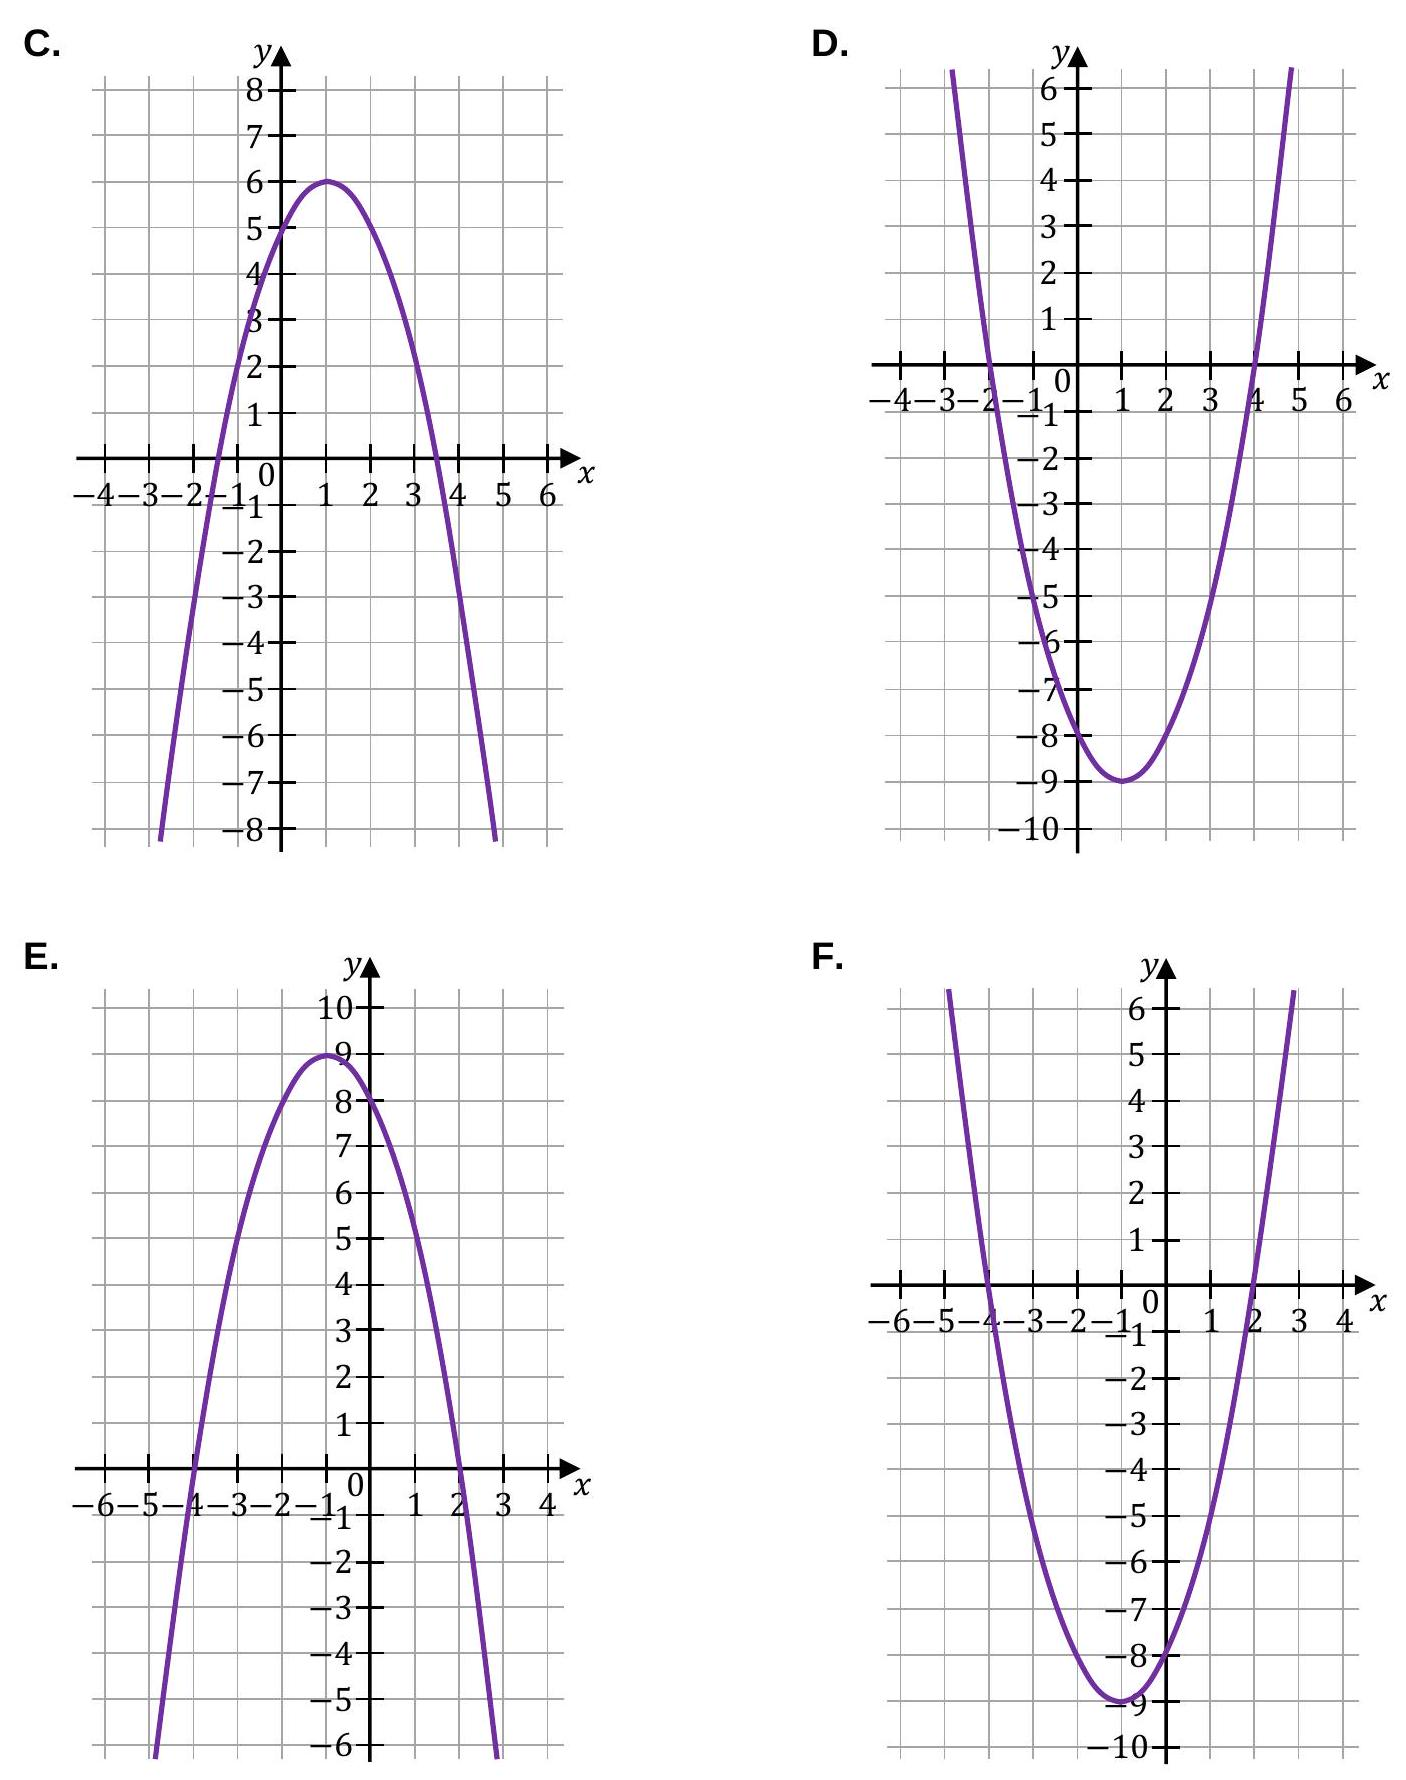
\includegraphics[max width=\textwidth, center]{2024_11_21_daeb5e5efb43dd4cb535g-15(1)}

Brudnopis\\

\includegraphics[max width=\textwidth, center]{2024_11_21_daeb5e5efb43dd4cb535g-15}

Zadanie 15. (0-1) 미미\\
Ciąg \(\left(a_{n}\right)\) jest określony wzorem \(a_{n}=(-1)^{n} \cdot(n-5)\) dla każdej liczby naturalnej \(n \geq 1\).

Oceń prawdziwość poniższych stwierdzeń. Wybierz P, jeśli stwierdzenie jest prawdziwe, albo F - jeśli jest fałszywe.

\begin{center}
\begin{tabular}{|l|c|c|}
\hline
\begin{tabular}{l}
Pierwszy wyraz ciągu \(\left(a_{n}\right)\) jest dwa razy większy od trzeciego wyrazu tego \\
ciągu. \\
\end{tabular} & \(\mathbf{P}\) & \(\mathbf{F}\) \\
\hline
Wszystkie wyrazy ciągu \(\left(a_{n}\right)\) są dodatnie. & \(\mathbf{P}\) & \(\mathbf{F}\) \\
\hline
\end{tabular}
\end{center}

\begin{center}
\begin{tabular}{|c|c|c|c|c|c|c|c|c|c|c|c|c|c|c|c|c|c|c|c|c|c|c|}
\hline
 & Brudn & nopis &  &  &  &  &  &  &  &  &  &  &  &  &  &  &  &  &  &  &  &  \\
\hline
 &  &  &  &  &  &  &  &  &  &  &  &  &  &  &  &  &  &  &  &  &  &  \\
\hline
 &  &  &  &  &  &  &  &  &  &  &  &  &  &  &  &  &  &  &  &  &  &  \\
\hline
 &  &  &  &  &  &  &  &  &  &  &  &  &  &  &  &  &  &  &  &  &  &  \\
\hline
 &  &  &  &  &  &  &  &  &  &  &  &  &  &  &  &  &  &  &  &  &  &  \\
\hline
 &  &  &  &  &  &  &  &  &  &  &  &  &  &  &  &  &  &  &  &  &  &  \\
\hline
 &  &  &  &  &  &  &  &  &  &  &  &  &  &  &  &  &  &  &  &  &  &  \\
\hline
 &  &  &  &  &  &  &  &  &  &  &  &  &  &  &  &  &  &  &  &  &  &  \\
\hline
 &  &  &  &  &  &  &  &  &  &  &  &  &  &  &  &  &  &  &  &  &  &  \\
\hline
\end{tabular}
\end{center}

Zadanie 16. (0-1) 미미\\
Trzywyrazowy ciąg (12, 6, \(2 m-1\) ) jest geometryczny.\\
Dokończ zdanie. Wybierz odpowiedź A albo B oraz odpowiedź 1., 2. albo 3.\\
Ten ciąg jest

\begin{center}
\begin{tabular}{|l|l|l|l|c|}
\hline
A. & rosnący &  & 1. & \(m=\frac{1}{2}\) \\
\cline { 4 - 4 }
 &  & oraz & 2. & \(m=2\) \\
\hline
B. & malejący &  & 3. & \(m=3\) \\
\hline
\end{tabular}
\end{center}

\begin{center}
\begin{tabular}{|c|c|c|c|c|c|c|c|c|c|c|c|c|c|c|c|c|c|c|c|c|c|c|c|}
\hline
\multicolumn{5}{|l|}{Brudnopis} &  &  &  &  &  &  &  &  &  &  &  &  &  &  &  &  &  &  &  \\
\hline
 &  &  &  &  &  &  &  &  &  &  &  &  &  &  &  &  &  &  &  &  &  &  &  \\
\hline
 &  &  &  &  &  &  &  &  &  &  &  &  &  &  &  &  &  &  &  &  &  &  &  \\
\hline
 &  &  &  &  &  &  &  &  &  &  &  &  &  &  &  &  &  &  &  &  &  &  &  \\
\hline
 &  &  &  &  &  &  &  &  &  &  &  &  &  &  &  &  &  &  &  &  &  &  &  \\
\hline
 &  &  &  &  &  &  &  &  &  &  &  &  &  &  &  &  &  &  &  &  &  &  &  \\
\hline
 &  &  &  &  &  &  &  &  &  &  &  &  &  &  &  &  &  &  &  &  &  &  &  \\
\hline
 &  &  &  &  &  &  &  &  &  &  &  &  &  &  &  &  &  &  &  &  &  &  &  \\
\hline
 &  &  &  &  &  &  &  &  &  &  &  &  &  &  &  &  &  &  &  &  &  &  &  \\
\hline
\end{tabular}
\end{center}

Zadanie 17. (0-2)\\
Ciąg arytmetyczny \(\left(a_{n}\right)\) jest określony dla każdej liczby naturalnej \(n \geq 1\). Trzeci wyraz tego ciągu jest równy ( -1 ), a suma piętnastu początkowych kolejnych wyrazów tego ciągu jest równa (-165).

Oblicz różnicę tego ciągu. Zapisz obliczenia.\\

\includegraphics[max width=\textwidth, center]{2024_11_21_daeb5e5efb43dd4cb535g-17}

Zadanie 18. (0-2)\\
W kartezjańskim układzie współrzędnych \((x, y)\) zaznaczono kąt o mierze \(\alpha\) taki, że \(\operatorname{tg} \alpha=-3\) oraz \(90^{\circ}<\alpha<180^{\circ}\) (zobacz rysunek).\\
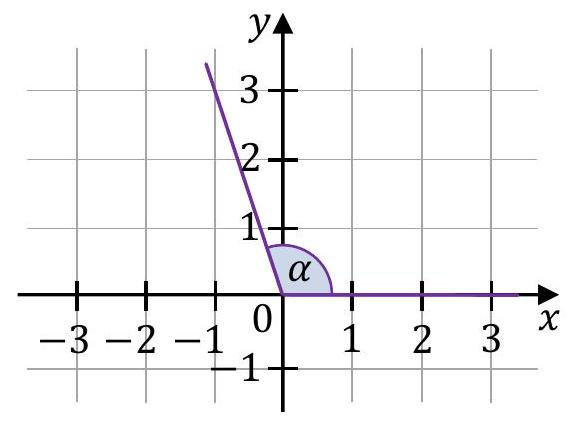
\includegraphics[max width=\textwidth, center]{2024_11_21_daeb5e5efb43dd4cb535g-18}

Uzupełnij zdanie. Wybierz dwie właściwe odpowiedzi spośród oznaczonych literami A-F i wpisz te litery w wykropkowanych miejscach.

Prawdziwe są zależności: \(\qquad\) oraz \(\qquad\) .\\
A. \(\sin \alpha<0\)\\
B. \(\sin \alpha \cdot \cos \alpha<0\)\\
C. \(\sin \alpha \cdot \cos \alpha>0\)\\
D. \(\cos \alpha>0\)\\
E. \(\sin \alpha=-\frac{1}{3} \cos \alpha\)\\
F. \(\sin \alpha=-3 \cos \alpha\)

\begin{center}
\begin{tabular}{|c|c|c|c|c|c|c|c|c|c|c|c|c|c|c|c|c|c|c|c|c|c|c|c|}
\hline
\multicolumn{4}{|l|}{Brudnopis} &  &  &  &  &  &  &  &  &  &  &  &  &  &  &  &  &  &  &  &  \\
\hline
 &  &  &  &  &  &  &  &  &  &  &  &  &  &  &  &  &  &  &  &  &  &  &  \\
\hline
 &  &  &  &  &  &  &  &  &  &  &  &  &  &  &  &  &  &  &  &  &  &  &  \\
\hline
 &  &  &  &  &  &  &  &  &  &  &  &  &  &  &  &  &  &  &  &  &  &  &  \\
\hline
 &  &  &  &  &  &  &  &  &  &  &  &  &  &  &  &  &  &  &  &  &  &  &  \\
\hline
 &  &  &  &  &  &  &  &  &  &  &  &  &  &  &  &  &  &  &  &  &  &  &  \\
\hline
 &  &  &  &  &  &  &  &  &  &  &  &  &  &  &  &  &  &  &  &  &  &  &  \\
\hline
 &  &  &  &  &  &  &  &  &  &  &  &  &  &  &  &  &  &  &  &  &  &  &  \\
\hline
\end{tabular}
\end{center}

\section*{Zadanie 19. (0-1) 마미}
Dokończ zdanie. Wybierz właściwą odpowiedź spośród podanych.\\
Liczba \(\sin ^{3} 20^{\circ}+\cos ^{2} 20^{\circ} \cdot \sin 20^{\circ}\) jest równa\\
A. \(\cos 20^{\circ}\)\\
B. \(\sin 20^{\circ}\)\\
C. \(\operatorname{tg} 20^{\circ}\)\\
D. \(\sin 20^{\circ} \cdot \cos 20^{\circ}\)

\begin{center}
\begin{tabular}{|c|c|c|c|c|c|c|c|c|c|c|c|c|c|c|c|c|c|c|c|c|c|c|c|c|c|c|}
\hline
\multicolumn{5}{|l|}{Brudnopis} &  &  &  &  &  &  &  &  &  &  &  &  &  &  &  &  &  &  &  &  &  &  \\
\hline
 &  &  &  &  &  &  &  &  &  &  &  &  &  &  &  &  &  &  &  &  &  &  &  &  &  &  \\
\hline
 &  &  &  &  &  &  &  &  &  &  &  &  &  &  &  &  &  &  &  &  &  &  &  &  &  &  \\
\hline
 &  &  &  &  &  &  &  &  &  &  &  &  &  &  &  &  &  &  &  &  &  &  &  &  &  &  \\
\hline
 &  &  &  &  &  &  &  &  &  &  &  &  &  &  &  &  &  &  &  &  &  &  &  &  &  &  \\
\hline
 &  &  &  &  &  &  &  &  &  &  &  &  &  &  &  &  &  &  &  &  &  &  &  &  &  &  \\
\hline
\end{tabular}
\end{center}

\section*{Zadanie 20. (0-1) 畺}
Dany jest trójkąt \(K L M\), w którym \(|K M|=a,|L M|=b\) oraz \(a \neq b\). Dwusieczna kąta \(K M L\) przecina bok \(K L\) w punkcie \(N\) takim, że \(|K N|=c,|N L|=d\) oraz \(|M N|=e\) (zobacz rysunek).\\
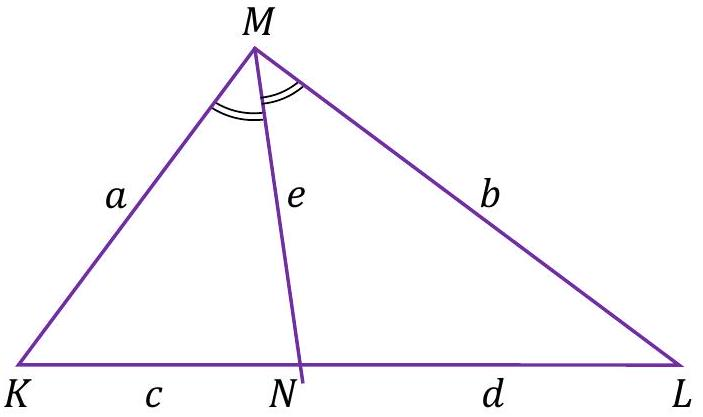
\includegraphics[max width=\textwidth, center]{2024_11_21_daeb5e5efb43dd4cb535g-19(1)}

Dokończ zdanie. Wybierz właściwą odpowiedź spośród podanych.

W trójkącie \(K L M\) prawdziwa jest równość\\
A. \(a \cdot b=c \cdot d\)\\
B. \(a \cdot d=b \cdot c\)\\
C. \(a \cdot c=b \cdot d\)\\
D. \(a \cdot b=e \cdot e\)

\begin{center}
\begin{tabular}{|c|c|c|c|c|c|c|c|c|c|c|c|c|c|c|c|c|c|c|c|c|c|c|c|c|c|c|c|}
\hline
\multicolumn{5}{|l|}{Brudnopis} &  &  &  &  &  &  &  &  &  &  &  &  &  &  &  &  &  &  &  &  &  &  &  \\
\hline
 &  &  &  &  &  &  &  &  &  &  &  &  &  &  &  &  &  &  &  &  &  &  &  &  &  &  &  \\
\hline
 &  &  &  &  &  &  &  &  &  &  &  &  &  &  &  &  &  &  &  &  &  &  &  &  &  &  &  \\
\hline
 &  &  &  &  &  &  &  &  &  &  &  &  &  &  &  &  &  &  &  &  &  &  &  &  &  &  &  \\
\hline
 &  &  &  &  &  &  &  &  &  &  &  &  &  &  &  &  &  &  &  &  &  &  &  &  &  &  &  \\
\hline
 &  &  &  &  &  &  &  &  &  &  &  &  &  &  &  &  &  &  &  &  &  &  &  &  &  &  &  \\
\hline
 &  &  &  &  &  &  &  &  &  &  &  &  &  &  &  &  &  &  &  &  &  &  &  &  &  &  &  \\
\hline
 &  &  &  &  &  &  &  &  &  &  &  &  &  &  &  &  &  &  &  &  &  &  &  &  &  &  &  \\
\hline
\end{tabular}
\end{center}

\section*{Zadanie 21. (0-1)}
Dany jest równoległobok o bokach długości 3 i 4 oraz o kącie między nimi o mierze \(120^{\circ}\).

Dokończ zdanie. Wybierz właściwą odpowiedź spośród podanych.

Pole tego równoległoboku jest równe\\
A. 12\\
B. \(12 \sqrt{3}\)\\
C. 6\\
D. \(6 \sqrt{3}\)

\begin{center}
\begin{tabular}{|c|c|c|c|c|c|c|c|c|c|c|c|c|c|c|c|c|c|c|c|c|c|c|c|c|c|c|c|c|c|c|}
\hline
 & d & op &  &  &  &  &  &  &  &  &  &  &  &  &  &  &  &  &  &  &  &  &  &  &  &  &  &  &  &  \\
\hline
 &  &  &  &  &  &  &  &  &  &  &  &  &  &  &  &  &  &  &  &  &  &  &  &  &  &  &  &  &  &  \\
\hline
 &  &  &  &  &  &  &  &  &  &  &  &  &  &  &  &  &  &  &  &  &  &  &  &  &  &  &  &  &  &  \\
\hline
到 &  &  &  &  &  &  &  &  &  &  &  &  &  &  &  &  &  &  &  &  &  &  &  &  &  &  &  &  &  &  \\
\hline
 &  &  &  &  &  &  &  &  &  &  &  &  &  &  &  &  &  &  &  &  &  &  &  &  &  &  &  &  &  &  \\
\hline
 &  &  &  &  &  &  &  &  &  &  &  &  &  &  &  &  &  &  &  &  &  &  &  &  &  &  &  &  &  &  \\
\hline
 &  &  &  &  &  &  &  &  &  &  &  &  &  &  &  &  &  &  &  &  &  &  &  &  &  &  &  &  &  &  \\
\hline
 &  &  &  &  &  &  &  &  &  &  &  &  &  &  &  &  &  &  &  &  &  &  &  &  &  &  &  &  &  & 
\includegraphics[max width=\textwidth]{2024_11_21_daeb5e5efb43dd4cb535g-19}
 \\
\hline
\end{tabular}
\end{center}

Zadanie 22. (0-1) 回\\
W trójkącie \(A B C\), wpisanym w okrąg o środku w punkcie \(S\), kąt \(A C B\) ma miarę \(42^{\circ}\) (zobacz rysunek).\\
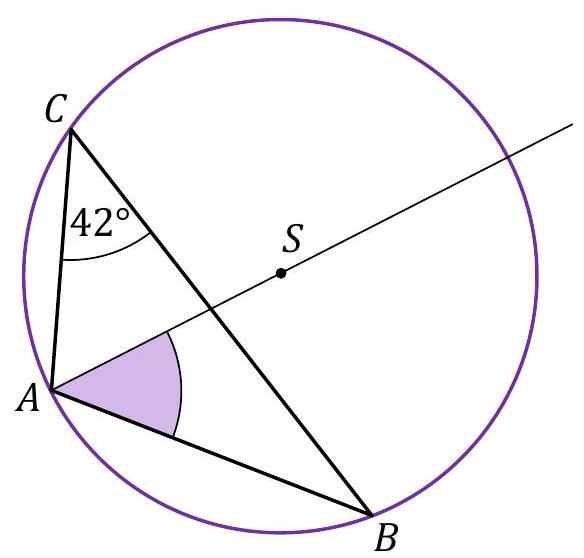
\includegraphics[max width=\textwidth, center]{2024_11_21_daeb5e5efb43dd4cb535g-20}

Dokończ zdanie. Wybierz właściwą odpowiedź spośród podanych.

Miara kąta ostrego \(B A S\) jest równa\\
A. \(42^{\circ}\)\\
B. \(45^{\circ}\)\\
C. \(48^{\circ}\)\\
D. \(69^{\circ}\)

\begin{center}
\begin{tabular}{|c|c|c|c|c|c|c|c|c|c|c|c|c|c|c|c|c|c|c|c|c|c|c|c|c|c|}
\hline
\multicolumn{4}{|l|}{Brudnopis} &  &  &  &  &  &  &  &  &  &  &  &  &  &  &  &  &  &  &  &  &  &  \\
\hline
 &  &  &  &  &  &  &  &  &  &  &  &  &  &  &  &  &  &  &  &  &  &  &  &  &  \\
\hline
 &  &  &  &  &  &  &  &  &  &  &  &  &  &  &  &  &  &  &  &  &  &  &  &  &  \\
\hline
 &  &  &  &  &  &  &  &  &  &  &  &  &  &  &  &  &  &  &  &  &  &  &  &  &  \\
\hline
 &  &  &  &  &  &  &  &  &  &  &  &  &  &  &  &  &  &  &  &  &  &  &  &  &  \\
\hline
\end{tabular}
\end{center}

\section*{Zadanie 23. (0-1) 回}
W kartezjańskim układzie współrzędnych \((x, y)\) proste \(k\) oraz \(l\) są określone równaniami

\[
\begin{aligned}
& k: y=(m+1) x+7 \\
& l: y=-2 x+7
\end{aligned}
\]

Dokończ zdanie. Wybierz właściwą odpowiedź spośród podanych.

Proste \(k\) oraz \(l\) są prostopadłe, gdy liczba \(m\) jest równa\\
A. \(\left(-\frac{1}{2}\right)\)\\
B. \(\frac{1}{2}\)\\
C. \((-3)\)\\
D. 1\\

\includegraphics[max width=\textwidth, center]{2024_11_21_daeb5e5efb43dd4cb535g-20(1)}

Zadanie 24. (0-2)\\
W kartezjańskim układzie współrzędnych \((x, y)\) dany jest równoległobok \(A B C D\), w którym \(A=(-2,6)\) oraz \(B=(10,2)\). Przekątne \(A C\) oraz \(B D\) tego równoległoboku przecinają się w punkcie \(P=(6,7)\).

Oblicz długość boku BC tego równoległoboku. Zapisz obliczenia.

\begin{center}
\begin{tabular}{|c|c|c|c|c|c|c|c|c|c|c|c|c|c|c|c|c|c|c|c|c|c|}
\hline
 &  &  &  &  &  &  &  &  &  &  &  &  &  &  &  &  &  &  &  &  &  \\
\hline
 &  &  &  &  &  &  &  &  &  &  &  &  &  &  &  &  &  &  &  &  &  \\
\hline
 &  &  &  &  &  &  &  &  &  &  &  &  &  &  &  &  &  &  &  &  &  \\
\hline
 &  &  &  &  &  &  &  &  &  &  &  &  &  &  &  &  &  &  &  &  &  \\
\hline
 &  &  &  &  &  &  &  &  &  &  &  &  &  &  &  &  &  &  &  &  &  \\
\hline
 &  &  &  &  &  &  &  &  &  &  &  &  &  &  &  &  &  &  &  &  &  \\
\hline
 &  &  &  &  &  &  &  &  &  &  &  &  &  &  &  &  &  &  &  &  &  \\
\hline
 &  &  &  &  &  &  &  &  &  &  &  &  &  &  &  &  &  &  &  &  &  \\
\hline
 &  &  &  &  &  &  &  &  &  &  &  &  &  &  &  &  &  &  &  &  &  \\
\hline
 &  &  &  &  &  &  &  &  &  &  &  &  &  &  &  &  &  &  &  &  &  \\
\hline
 &  &  &  &  &  &  &  &  &  &  &  &  &  &  &  &  &  &  &  &  &  \\
\hline
 &  &  &  &  &  &  &  &  &  &  &  &  &  &  &  &  &  &  &  &  &  \\
\hline
 &  &  &  &  &  &  &  &  &  &  &  &  &  &  &  &  &  &  &  &  &  \\
\hline
 &  &  &  &  &  &  &  &  &  &  &  &  &  &  &  &  &  &  &  &  &  \\
\hline
 &  &  &  &  &  &  &  &  &  &  &  &  &  &  &  &  &  &  &  &  &  \\
\hline
 &  &  &  &  &  &  &  &  &  &  &  &  &  &  &  &  &  &  &  &  &  \\
\hline
 &  &  &  &  &  &  &  &  &  &  &  &  &  &  &  &  &  &  &  &  &  \\
\hline
 &  &  &  &  &  &  &  &  &  &  &  &  &  &  &  &  &  &  &  &  &  \\
\hline
 &  &  &  &  &  &  &  &  &  &  &  &  &  &  &  &  &  &  &  &  &  \\
\hline
 &  &  &  &  &  &  &  &  &  &  &  &  &  &  &  &  &  &  &  &  &  \\
\hline
 &  &  &  &  &  &  &  &  &  &  &  &  &  &  &  &  &  &  &  &  &  \\
\hline
 &  &  &  &  &  &  &  &  &  &  &  &  &  &  &  &  &  &  &  &  &  \\
\hline
 &  &  &  &  &  &  &  &  &  &  &  &  &  &  &  &  &  &  &  &  &  \\
\hline
 &  &  &  &  &  &  &  &  &  &  &  &  &  &  &  &  &  &  &  &  &  \\
\hline
 &  &  &  &  &  &  &  &  &  &  &  &  &  &  &  &  &  &  &  &  &  \\
\hline
 &  &  &  &  &  &  &  &  &  &  &  &  &  &  &  &  &  &  &  &  &  \\
\hline
 &  &  &  &  &  &  &  &  &  &  &  &  &  &  &  &  &  &  &  &  &  \\
\hline
 &  &  &  &  &  &  &  &  &  &  &  &  &  &  &  &  &  &  &  &  &  \\
\hline
 &  &  &  &  &  &  &  &  &  &  &  &  &  &  &  &  &  &  &  &  &  \\
\hline
 &  &  &  &  &  &  &  &  &  &  &  &  &  &  &  &  &  &  &  &  &  \\
\hline
 &  &  &  &  &  &  &  &  &  &  &  &  &  &  &  &  &  &  &  &  &  \\
\hline
 &  &  &  &  &  &  &  &  &  &  &  &  &  &  &  &  &  &  &  &  &  \\
\hline
 &  &  &  &  &  &  &  &  &  &  &  &  &  &  &  &  &  &  &  &  &  \\
\hline
 &  &  &  &  &  &  &  &  &  &  &  &  &  &  &  &  &  &  &  &  &  \\
\hline
 &  &  &  &  &  &  &  &  &  &  &  &  &  &  &  &  &  &  &  &  &  \\
\hline
 &  &  &  &  &  &  &  &  &  &  &  &  &  &  &  &  &  &  &  &  &  \\
\hline
 &  &  &  &  &  &  &  &  &  &  &  &  &  &  &  &  &  &  &  &  &  \\
\hline
 &  &  &  &  &  &  &  &  &  &  &  &  &  &  &  &  &  &  &  &  &  \\
\hline
 &  &  &  &  &  &  &  &  &  &  &  &  &  &  &  &  &  &  &  &  &  \\
\hline
 &  &  &  &  &  &  &  &  &  &  &  &  &  &  &  &  &  &  &  &  &  \\
\hline
 &  &  &  &  &  &  &  &  &  &  &  &  &  &  &  &  &  &  &  &  &  \\
\hline
\end{tabular}
\end{center}

\section*{Zadanie 25.}
Wysokość graniastosłupa prawidłowego sześciokątnego jest równa 6 (zobacz rysunek). Pole podstawy tego graniastosłupa jest równe \(15 \sqrt{3}\).\\
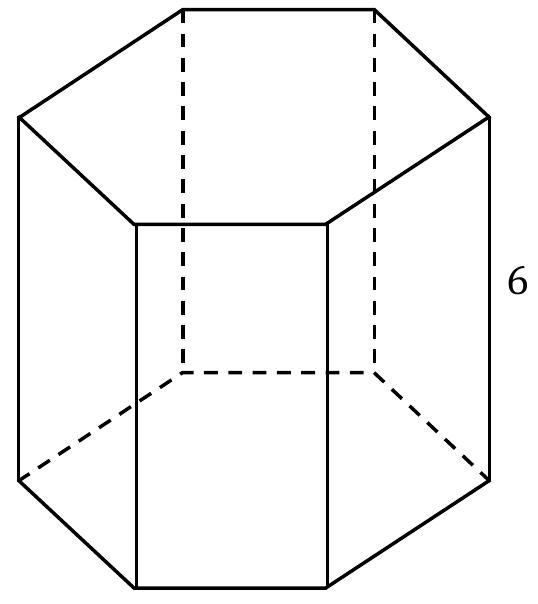
\includegraphics[max width=\textwidth, center]{2024_11_21_daeb5e5efb43dd4cb535g-22}

Zadanie 25.1. (0-1)\\
Dokończ zdanie. Wybierz właściwą odpowiedź spośród podanych.\\
Pole ¡ednej ściany bocznej tego graniastosłupa jest równe\\
A. \(36 \sqrt{10}\)\\
B. 60\\
C. \(6 \sqrt{10}\)\\
D. 360\\

\includegraphics[max width=\textwidth, center]{2024_11_21_daeb5e5efb43dd4cb535g-22(1)}

Zadanie 25.2. (0-1) 미미\\
Dokończ zdanie. Wybierz właściwą odpowiedź spośród podanych.\\
Kąt nachylenia najdłuższej przekątnej graniastosłupa prawidłowego sześciokątnego do płaszczyzny podstawy jest zaznaczony na rysunku\\
A.\\
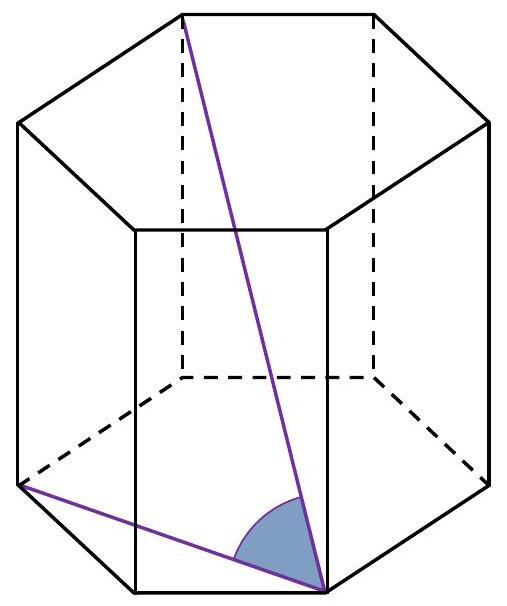
\includegraphics[max width=\textwidth, center]{2024_11_21_daeb5e5efb43dd4cb535g-23(2)}\\
B.\\
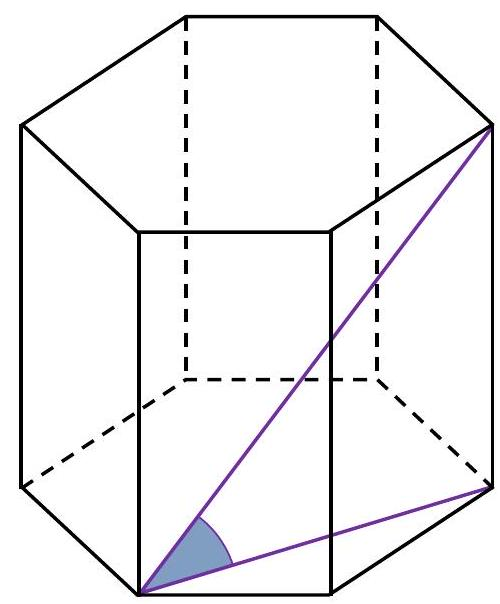
\includegraphics[max width=\textwidth, center]{2024_11_21_daeb5e5efb43dd4cb535g-23(3)}\\
C.\\
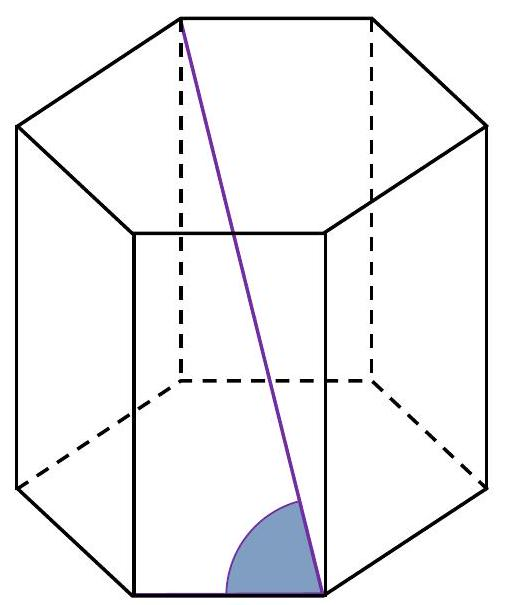
\includegraphics[max width=\textwidth, center]{2024_11_21_daeb5e5efb43dd4cb535g-23(1)}\\
D.\\
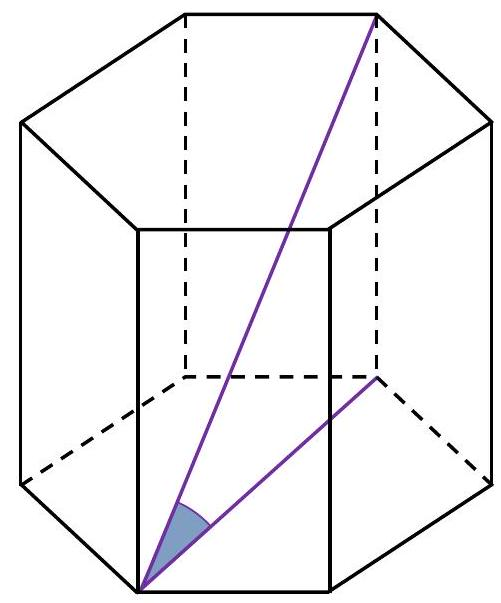
\includegraphics[max width=\textwidth, center]{2024_11_21_daeb5e5efb43dd4cb535g-23}

\begin{center}
\begin{tabular}{|c|c|c|c|c|c|c|c|c|c|c|c|c|c|c|c|c|c|c|c|c|c|c|}
\hline
\multicolumn{4}{|l|}{Brudnopis} &  &  &  &  &  &  &  &  &  &  &  &  &  &  &  &  &  &  &  \\
\hline
 &  &  &  &  &  &  &  &  &  &  &  &  &  &  &  &  &  &  &  &  &  &  \\
\hline
 &  &  &  &  &  &  &  &  &  &  &  &  &  &  &  &  &  &  &  &  &  &  \\
\hline
 &  &  &  &  &  &  &  &  &  &  &  &  &  &  &  &  &  &  &  &  &  &  \\
\hline
 &  &  &  &  &  &  &  &  &  &  &  &  &  &  &  &  &  &  &  &  &  &  \\
\hline
 &  &  &  &  &  &  &  &  &  &  &  &  &  &  &  &  &  &  &  &  &  &  \\
\hline
 &  &  &  &  &  &  &  &  &  &  &  &  &  &  &  &  &  &  &  &  &  &  \\
\hline
 &  &  &  &  &  &  &  &  &  &  &  &  &  &  &  &  &  &  &  &  &  &  \\
\hline
 &  &  &  &  &  &  &  &  &  &  &  &  &  &  &  &  &  &  &  &  &  &  \\
\hline
 &  &  &  &  &  &  &  &  &  &  &  &  &  &  &  &  &  &  &  &  &  &  \\
\hline
 &  &  &  &  &  &  &  &  &  &  &  &  &  &  &  &  &  &  &  &  &  &  \\
\hline
 &  &  &  &  &  &  &  &  &  &  &  &  &  &  &  &  &  &  &  &  &  &  \\
\hline
\end{tabular}
\end{center}

Zadanie 26. (0-1)\\
Ostrosłup \(F_{1}\) jest podobny do ostrosłupa \(F_{2}\).\\
Objętość ostrosłupa \(F_{1}\) jest równa 64.\\
Objętość ostrosłupa \(F_{2}\) jest równa 512.

Uzupełnij poniższe zdanie. Wpisz odpowiednią liczbę w wykropkowanym miejscu tak, aby zdanie było prawdziwe.

Stosunek pola powierzchni całkowitej ostrosłupa \(F_{2}\) do pola powierzchni całkowitej ostrosłupa \(F_{1}\) jest równy \(\qquad\)

\begin{center}
\begin{tabular}{|c|c|c|c|c|c|c|c|c|c|c|c|c|c|c|c|c|c|c|c|c|c|}
\hline
\multicolumn{4}{|l|}{Brudnopis} &  &  &  &  &  &  &  &  &  &  &  &  &  &  &  &  &  &  \\
\hline
 &  &  &  &  &  &  &  &  &  &  &  &  &  &  &  &  &  &  &  &  &  \\
\hline
 &  &  &  &  &  &  &  &  &  &  &  &  &  &  &  &  &  &  &  &  &  \\
\hline
 &  &  &  &  &  &  &  &  &  &  &  &  &  &  &  &  &  &  &  &  &  \\
\hline
 &  &  &  &  &  &  &  &  &  &  &  &  &  &  &  &  &  &  &  &  &  \\
\hline
 &  &  &  &  &  &  &  &  &  &  &  &  &  &  &  &  &  &  &  &  &  \\
\hline
 &  &  &  &  &  &  &  &  &  &  &  &  &  &  &  &  &  &  &  &  &  \\
\hline
 &  &  &  &  &  &  &  &  &  &  &  &  &  &  &  &  &  &  &  &  &  \\
\hline
 &  &  &  &  &  &  &  &  &  &  &  &  &  &  &  &  &  &  &  &  &  \\
\hline
 &  &  &  &  &  &  &  &  &  &  &  &  &  &  &  &  &  &  &  &  &  \\
\hline
 &  &  &  &  &  &  &  &  &  &  &  &  &  &  &  &  &  &  &  &  &  \\
\hline
 &  &  &  &  &  &  &  &  &  &  &  &  &  &  &  &  &  &  &  &  &  \\
\hline
\end{tabular}
\end{center}

\section*{Zadanie 27. (0-1) 미미}
Rozważamy wszystkie kody czterocyfrowe utworzone tylko z cyfr 1, 3, 6, 8, przy czym w każdym kodzie każda z tych cyfr występuje dokładnie jeden raz.

Dokończ zdanie. Wybierz właściwą odpowiedź spośród podanych.\\
Liczba wszystkich takich kodów jest równa\\
A. 4\\
B. 10\\
C. 24\\
D. 16\\

\includegraphics[max width=\textwidth, center]{2024_11_21_daeb5e5efb43dd4cb535g-24}

Zadanie 28. (0-1) 回\\
Średnia arytmetyczna trzech liczb: \(a, b, c\), jest równa 9.\\
Dokończ zdanie. Wybierz właściwą odpowiedź spośród podanych.

Średnia arytmetyczna sześciu liczb: \(a, a, b, b, c, c\), jest równa\\
A. 9\\
B. 6\\
C. 4,5\\
D. 18

\begin{center}
\begin{tabular}{|c|c|c|c|c|c|c|c|c|c|c|c|c|c|c|c|c|c|c|c|c|c|c|c|c|c|c|c|c|c|c|}
\hline
\multicolumn{5}{|l|}{Brudnopis} &  &  &  &  &  &  &  &  &  &  &  &  &  &  &  &  &  &  &  &  &  &  &  &  &  &  \\
\hline
 &  &  &  &  &  &  &  &  &  &  &  &  &  &  &  &  &  &  &  &  &  &  &  &  &  &  &  &  &  &  \\
\hline
 &  &  &  &  &  &  &  &  &  &  &  &  &  &  &  &  &  &  &  &  &  &  &  &  &  &  &  &  &  &  \\
\hline
 &  &  &  &  &  &  &  &  &  &  &  &  &  &  &  &  &  &  &  &  &  &  &  &  &  &  &  &  &  &  \\
\hline
 &  &  &  &  &  &  &  &  &  &  &  &  &  &  &  &  &  &  &  &  &  &  &  &  &  &  &  &  &  &  \\
\hline
 &  &  &  &  &  &  &  &  &  &  &  &  &  &  &  &  &  &  &  &  &  &  &  &  &  &  &  &  &  &  \\
\hline
\end{tabular}
\end{center}

\section*{Zadanie 29. (0-1)}
Na diagramie przedstawiono wyniki sprawdzianu z matematyki w pewnej klasie maturalnej. Na osi poziomej podano oceny, które uzyskali uczniowie tej klasy, a na osi pionowej podano liczbę uczniów, którzy otrzymali daną ocenę.\\
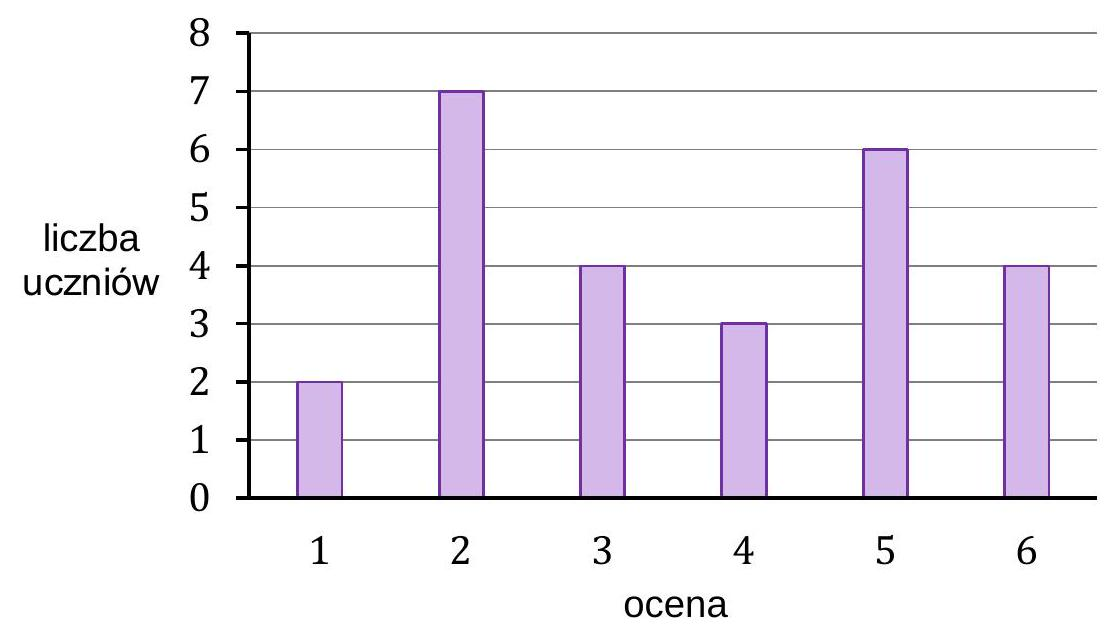
\includegraphics[max width=\textwidth, center]{2024_11_21_daeb5e5efb43dd4cb535g-25(1)}

Dokończ zdanie. Wybierz właściwą odpowiedź spośród podanych.\\
Mediana ocen uzyskanych z tego sprawdzianu przez uczniów tej klasy jest równa\\
A. 4,5\\
B. 4\\
C. 3,5\\
D. 3\\

\includegraphics[max width=\textwidth, center]{2024_11_21_daeb5e5efb43dd4cb535g-25}

Zadanie 30. (0-2)\\
Dany jest pięcioelementowy zbiór \(K=\{5,6,7,8,9\}\). Wylosowanie każdej liczby z tego zbioru jest jednakowo prawdopodobne. Ze zbioru \(K\) losujemy ze zwracaniem kolejno dwa razy po jednej liczbie i zapisujemy je w kolejności losowania.

Oblicz prawdopodobieństwo zdarzenia \(A\) polegającego na tym, że suma wylosowanych liczb jest liczbą parzystą. Zapisz obliczenia.\\

\includegraphics[max width=\textwidth, center]{2024_11_21_daeb5e5efb43dd4cb535g-26}

Zadanie 31. (0-4)\\
W schronisku dla zwierząt, na płaskiej powierzchni, należy zbudować ogrodzenie z siatki wydzielające trzy identyczne wybiegi o wspólnych ścianach wewnętrznych.\\
Podstawą każdego z tych trzech wybiegów jest prostokąt (jak pokazano na rysunku). Do wykonania tego ogrodzenia należy zużyć 36 metrów bieżących siatki.

Schematyczny rysunek trzech wybiegów (widok z góry). Linią przerywaną zaznaczono siatkę.\\
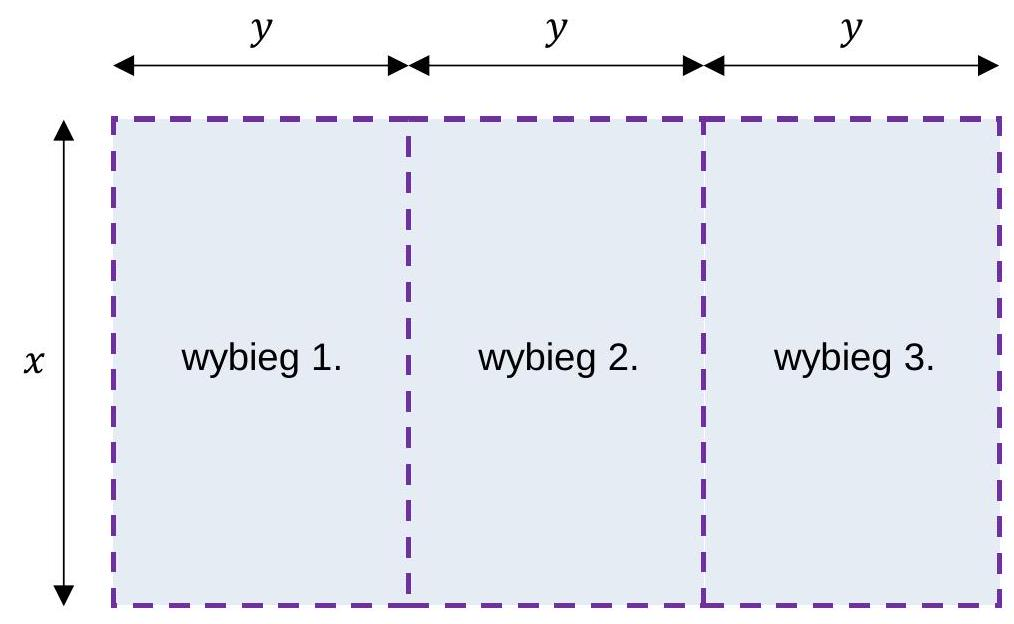
\includegraphics[max width=\textwidth, center]{2024_11_21_daeb5e5efb43dd4cb535g-27}

Oblicz wymiary \(x\) oraz \(y\) jednego wybiegu, przy których suma pól podstaw tych trzech wybiegów będzie największa. W obliczeniach pomiń szerokość wejścia na każdy z wybiegów. Zapisz obliczenia.\\

\includegraphics[max width=\textwidth, center]{2024_11_21_daeb5e5efb43dd4cb535g-27(1)}\\
\(\square\)\\

\includegraphics[max width=\textwidth, center]{2024_11_21_daeb5e5efb43dd4cb535g-28}

BRUDNOPIS (nie podlega ocenie)\\

\includegraphics[max width=\textwidth, center]{2024_11_21_daeb5e5efb43dd4cb535g-29}\\

\includegraphics[max width=\textwidth, center]{2024_11_21_daeb5e5efb43dd4cb535g-30}

\section*{MATEMATYKA}
\section*{Poziom podstawowy}
Formuła 2023

\section*{MATEMATYKA}
\section*{Poziom podstawowy}
Formuła 2023

\section*{MATEMATYKA}
\section*{Poziom podstawowy}
Formuła 2023


\end{document}